\documentclass[graybox, envcountchap]{Template/svmult}


\usepackage{natbib}
\usepackage{mathptmx}        % selects Times Roman as basic font
\usepackage{amsmath}
\usepackage{amssymb}
\usepackage{color}
\usepackage{colortbl}        % row colouring in tables
\usepackage{rotating}        % sidewaystable for wide tables
\definecolor{rowhl}{rgb}{0.95,0.92,0.84} % highlight tint (matches figures)
\usepackage{helvet}          % selects Helvetica as sans-serif font
\usepackage{courier}         % selects Courier as typewriter font
\usepackage{dirtree}
%\usepackage{type1cm}        % activate if the above 3 fonts are
                             % not available on your system

\usepackage{makeidx}        % allows index generation
\usepackage{graphicx}        % standard LaTeX graphics tool
                                            % when including figure files
\usepackage{subfig}
\usepackage{array}           % \arraybackslash for p{} columns in the table

\usepackage{multicol}        % used for the two-column index
\usepackage[bottom]{footmisc}% places footnotes at page bottom

\usepackage{hyperref}        %for hyperlinks
\hypersetup{colorlinks=true,urlcolor=blue}

\usepackage[misc]{ifsym}

\makeindex             % used for the subject index
                       % please use the style svind.ist with
                       % your makeindex program


\begin{document}


%%%%%%%%%%%%%%%%%%%%%%%%%%%%%%%%%%%%%%%%%%%%%%%%%%%%%%%%%%%%%%%%%



\title{Machine Learning Techniques for Astrophysics and Cosmology: Graph Neural Networks}
% Use \titlerunning{Short Title} for an abbreviated version of
% your contribution title if the original one is too long
\titlerunning{Graph Neural Networks}
\author{Christian Kragh Jespersen}
\authorrunning{C. Kragh Jespersen}
\institute{Christian Kragh Jespersen (\Letter) \at Department of Astrophysical Sciences, Princeton University, Princeton, NJ 08544, USA, \email{ckragh@princeton.edu}}
\maketitle

\abstract{Modern astrophysics drowns not in data, but in relations. We seldom
measure an object alone; we measure how it sits among its neighbours --- a
galaxy in its environment, a halo in its history, a photon hit in a detector.
Graphs encode exactly these relations, and graph neural networks (GNNs) are the
learning algorithms built to respect them. This chapter argues, from first
principles, that GNNs are the natural instrument for physical data: they adapt
to the native geometry of the domain and the signal, they embed the symmetries
and the prior knowledge we already trust, and they stay flexible enough to fit
what we do not yet understand. We start from the geometry of learning, recover
the convolutional network and the transformer as special cases of a single
geometric blueprint, and then build the graph and the graph neural network from
the ground up. We survey applications across cosmology, galaxy formation,
dynamics, and instrumentation; we distil a set of best practices, including the
unfashionable question of when \emph{not} to reach for a graph; and we chart the
frontier. Throughout we prefer physical intuition to abstract machinery, on the
old conviction --- due to Helv\'etius --- that the knowledge of certain
principles readily supplies the knowledge of certain facts.}


%%%%%%%%%%%%%%%%%%%%%%%%%%%%%%%%%%%%%%%%%%%%%%%%%%%%%%%%%


\section{Introduction}
\label{sec:intro}

The history of physics is a story of geometry. Learning algorithms for the
physical world must therefore be grounded in geometry.\footnote{Graph theory
itself was born of a geometric puzzle: in 1736 Euler reduced the seven bridges
of K\"onigsberg to nodes and edges and proved the stroll impossible. Three
centuries on, the same abstraction describes the largest structures in the
Universe.} From the ellipses of Kepler, through the invariances of Galileo, to
the curved spacetime of Einstein, physics advances less by collecting facts than
by finding the symmetry that renders the facts inevitable. A theory earns our
trust when it states its laws in a form that no choice of coordinates, no
relabelling, and no idle rotation can disturb.

The natural sciences are, at heart, relational. We build theories not of
isolated objects but of the relations between them, and graphs hold precisely
this structure: objects become nodes, relations become edges. Such data
permeate the field. Merger trees record the assembly of a halo; the cosmic web
threads galaxies into filaments; a neutrino observatory scatters its sensors
through a kilometre of ice. None of these live on a regular grid, and forcing
them onto one invents a structure the data never had.

Graph neural networks belong to the modern family of \emph{geometric} deep
learning architectures, which harness relational inductive biases for functions
on arbitrary domains \citep{Bronstein2021_geometricDL_book}. They propagate
information along edges through parameterised message passing, and read out
node-, edge-, and graph-level quantities. The idea is older than the recent
enthusiasm suggests: recursive and recurrent precursors reach back to the late
1990s, and the message-passing view that organises this chapter has by now
absorbed convolutional networks and transformers as special cases
\citep{Velickovic2022_messagepassing_up}.

This chapter proceeds in three movements. We first develop the geometry of
learning and the blueprint that unifies its architectures
(Sect.~\ref{sec:geometry}). We then construct graphs and graph neural networks
from the ground up (Sects.~\ref{sec:graphs}--\ref{sec:gnn}). Finally we review
the astrophysical applications (Sect.~\ref{sec:applications}), set out best
practices (Sect.~\ref{sec:bestpractices}), and survey the frontier
(Sect.~\ref{sec:frontier}).


%%%%%%%%%%%%%%%%%%%%%%%%%%%%%%%%%%%%%%%%%%%%%%%%%%%%%%%%%


\section{Geometry and Deep Learning}
\label{sec:geometry}

\begin{quotation}
\noindent\textit{``La connaissance de certains principes supplée facilement à
la connaissance de certains faits.''} \\
\noindent (``The knowledge of certain principles readily supplies the knowledge
of certain facts.'') \\
\noindent\hfill --- Claude Adrien Helv\'etius
\end{quotation}

This section makes a promise in Helv\'etius's spirit: master a few principles,
and you can \emph{derive} --- rather than memorise --- the right architecture
for the problem in front of you. The recipe takes three inputs --- the problem
you pose, the signal you measure, and the domain on which it lives --- and
returns the symmetries to respect and the layers to stack. We separate the
geometry of the domain from that of the signal, fix the language of symmetry,
and then assemble the blueprint from which the convolutional network, the
transformer, and the graph neural network all descend.

\subsection{The geometry of the domain and of the signal}
\label{sec:domain-signal}

A learning problem hides two geometries, and good models respect both. The
first is the geometry of the \emph{domain} --- the support on which the data
live: a regular grid, a sphere, an irregular point cloud, a graph. The second is
the geometry of the \emph{signal} --- the structure of the field defined on that
support, which carries its own symmetries (a temperature is a scalar, a velocity
a vector, a shear a tensor, whatever grid we happen to sample them on).

The lesson repeats throughout this chapter, so we state it once and plainly:
choose the algorithm that respects the native geometry of both the domain and
the signal. Impose no symmetry the data lack, and discard none they possess. A
convolutional network presumes a regular grid; run it on a sphere or an
irregular detector and one must first voxelise, and so invent a translational
structure that is simply not there. Where the domain is genuinely irregular, a
graph is not a stylistic preference but the only faithful description.

% TODO: create this figure
\begin{figure}[t]
\includegraphics[width=\textwidth]{figures/TODO_domain_signal_geometry}% TODO: make own figure
\caption{TODO --- MAKE OWN VERSION. The two geometries of a learning problem:
the \emph{domain} (grid vs.\ sphere vs.\ point cloud vs.\ graph) and the
\emph{signal} living on it (scalar, vector, tensor field), with the algorithm
each admits.}
\label{fig:domain_signal}
\end{figure}

\subsection{Symmetries, invariances, and equivariances}
\label{sec:symmetries}

A \emph{symmetry} is a transformation that leaves some property untouched. The
physicist meets symmetries early: the result of an experiment does not depend on
where the bench stands, which way it faces, or when one runs it. The
transformations that preserve a structure form a \emph{group}, and how that
group acts on our data --- through linear maps called \emph{representations} ---
dictates how a sensible model must behave. We keep the formal account, with the
group axioms and the representation theory, to Appendix~\ref{app:symmetries};
here we need only two words.

A function is \emph{invariant} when the group action leaves its output
unchanged, and \emph{equivariant} when the output transforms in step with the
input. The distinction is the difference between a scalar and a vector. Rotate a
molecule: its total energy does not move (invariant), but the force on each atom
rotates with it (equivariant). The same split organises every prediction we make
on a graph, and we return to it in Sect.~\ref{sec:gnn}. Invariance, it is worth
noting, is simply the special case of equivariance in which the output carries
the trivial representation.

\subsection{The geometric blueprint, and the convolutional network it implies}
\label{sec:blueprint}

Almost every successful architecture is one recipe, applied to a different
domain and symmetry. Fix a domain $\Omega$ with symmetry group $G$ and assemble
four kinds of block, as set out in the blueprint of
\citet{Bronstein2021_geometricDL_book}.

\begin{svgraybox}
\textbf{The Geometric Deep Learning blueprint.} From a domain $\Omega$ with
symmetry group $G$, build:
\begin{itemize}
  \item a \textbf{$G$-equivariant layer} $B$, which mixes features in step with
        the symmetry, $B(g.x)=g.B(x)$;
  \item a pointwise \textbf{non-linearity} $\sigma$;
  \item an optional \textbf{local pooling (coarsening)} $P$, which shrinks the
        domain while it preserves the symmetry;
  \item a \textbf{global pooling} $A$, which reads out a $G$-\emph{invariant}
        answer, $A(g.x)=A(x)$.
\end{itemize}
Stack the equivariant blocks (with non-linearities and optional coarsening) and
finish with the invariant readout:
\[
  f \;=\; A \circ \sigma_J \circ B_J \circ P_{J-1}\circ\cdots\circ
          P_1 \circ \sigma_1 \circ B_1 .
\]
\end{svgraybox}

To see the recipe at work, derive the convolutional network. Since many readers
hold a firm intuition for images and a shakier one for graphs, we let the
familiar case lead. Demand three things \emph{a priori} of a model that acts on
an image: translational \emph{equivariance} of its internal operations, scale
separation, and translational \emph{invariance} of its output. The first
requirement is decisive. To insist that a local linear operation commute with
every shift forces it to share its weights across the image --- that is, to be a
\emph{convolution}. Scale separation, the premise that one may coarsen the signal
without loss of what matters, justifies the interleaved \emph{pooling} that
stacks these convolutions into a multiscale hierarchy; a dog stays a dog across
scales and small deformations. Demand finally that the \emph{output} ignore
position, and a single \emph{global pooling} delivers it. Reassembled, the parts
are nothing but the familiar convolutional network --- and exactly the blueprint
above, with the group set to translations.

The same recipe, with a different group and a different notion of locality, then
yields the rest. A transformer is the blueprint on a fully connected graph with
attention as a learned, soft adjacency; a deep set is the blueprint on a set,
the edgeless limit; a graph neural network is the blueprint on a graph with the
permutation group. We do not claim that a transformer simply \emph{is} a graph
neural network --- its positional encodings reinstate the order a
permutation-equivariant layer discards, and the difference matters --- only that
all of them descend from one geometric principle. The graph earns its central
place here not because it is fashionable, but because it is the humble, general
substrate from which the specialised successes fall out as corollaries.

\subsection{Where graph neural networks sit: the five Gs}
\label{sec:5gs}

Geometric deep learning surveys five families of domain --- grids, groups,
graphs, geodesics, and gauges, the ``five Gs''
\citep{Bronstein2021_geometricDL_book} --- and graphs are but one province of
that map. We mention the others only to place our subject within it; the same
blueprint specialises to each. Table~\ref{tab:gdl_architectures} collects the
common architectures as instances of the blueprint, and marks the one this
chapter pursues.

\begin{table}[t]
\caption{Common geometric architectures as instances of the geometric deep
learning blueprint, after \citet{Bronstein2021_geometricDL_book} (trimmed). The
GNN row --- the focus of this chapter --- is highlighted.}
\label{tab:gdl_architectures}
\centering\footnotesize\setlength{\tabcolsep}{4pt}
\begin{tabular}{lll>{\raggedright\arraybackslash}p{2.2cm}>{\raggedright\arraybackslash}p{2.6cm}>{\raggedright\arraybackslash}p{2.8cm}}
\hline\noalign{\smallskip}
Architecture & Domain $\Omega$ & Symmetry $G$ & Locality & Example (non-astro) & Example (astronomy) \\
\noalign{\smallskip}\svhline\noalign{\smallskip}
CNN           & Grid           & Translation            & local patch & image classification \citep{Krizhevsky2012_alexnet_imagenet} & galaxy morphology \citep{Dieleman2015_galaxymorphology_CNN} \\
Spherical CNN & Sphere         & Rotation $SO(3)$       & local cap   & omnidirectional vision \citep{Cohen2018_spherical_CNN} & weak-lensing maps \citep{Perraudin2019_deepsphere_spherical} \\
\rowcolor{rowhl}
GNN           & Graph          & Permutation $\Sigma_n$ & neighbours  & molecular properties \citep{Gilmer2017_MPNN_quantumchemistry} & merger trees \citep{Jespersen2022_mangrove} \\
Deep Sets     & Set            & Permutation $\Sigma_n$ & none        & point clouds \citep{Zaheer2017_deepsets} & cosmic voids \citep{Cranmer2021_histpool_deepsets} \\
Transformer   & Complete graph & Permutation $\Sigma_n$ & all-to-all  & language \citep{Vaswani2017_transformer_attention} & light curves \citep{DonosoOliva2023_astromer_transformer} \\
\noalign{\smallskip}\hline
\end{tabular}
\end{table}


%%%%%%%%%%%%%%%%%%%%%%%%%%%%%%%%%%%%%%%%%%%%%%%%%%%%%%%%%


\section{Graphs}
\label{sec:graphs}

Before we learn on a graph, we must say what a graph is, how we build one, and
when we have no choice but to use one. This section takes the three in turn: it
fixes the notation, it treats the adjacency matrix as the design choice it
really is, and it shows the astrophysical settings in which the graph is simply
inevitable. One point deserves emphasis at the outset: the graph picture earns
its keep even when no neural network touches it. A graph path-likelihood, for
instance, extracts galaxy-formation information from the structure of a layered
halo graph alone, with not a single learned weight in sight
\citep{Yang2026_halograph_likelihood_not_gnn}.

\subsection{Definitions and notation}
\label{sec:graph-defs}

We define a graph as the triple $G=(V,E,U)$. Here $V=\{\mathbf{v}_i\}_{i=1:N^v}$
is the set of node feature vectors; $E=\{(\mathbf{e}_k,r_k,s_k)\}$ is the set of
edge feature vectors, each tied to a receiver $r_k$ and a sender $s_k$; and $U$
is a global, graph-level feature vector. We follow the notation of
\citet{Battaglia2018_relational_GN}. The connectivity also admits a compact
description through the binary adjacency matrix $A$, where $A_{ij}=1$ marks an
edge. Real graphs are sparse, so in practice one stores not the dense $N\times
N$ matrix but the \emph{edge index} --- the two rows of sender and receiver
indices --- which is how message passing is actually computed.

A graph may be directed or undirected, and the physics of the relation should
decide which. Directed edges suit asymmetric, causal, or ordered relations: a
merger tree points forward in time, since to pass information backwards would
break causality. Undirected edges (a symmetric $A$) suit symmetric relations ---
spatial proximity, a chemical bond, a pairwise gravitational pull. The
\emph{neighbourhood} $\mathcal{N}(u)$ collects the nodes joined to $u$, and on it
rests the whole notion of locality that follows.

% TODO: create this figure
\begin{figure}[t]
\includegraphics[width=\textwidth]{figures/TODO_sketch_graphs_adjacency}% TODO: make own figure
\caption{TODO --- MAKE OWN VERSION (companion script to
\texttt{figures/computational\_modules.py}). A few sketch graphs --- a star, a
cycle, a complete graph --- with their dense adjacency matrices and the
equivalent sparse sender/receiver edge index.}
\label{fig:sketch_graphs}
\end{figure}

\subsection{Building the graph: the adjacency is a choice}
\label{sec:no-adjacency}

Often the graph arrives ready-made; just as often it does not, and we must
decide who connects to whom. There are four standard moves. We may \emph{impose}
an edge set from physical knowledge --- at a neutrino observatory, connect only
hits whose separation is consistent with a signal at or below the speed of light,
a causal constraint no honest edge may violate. We may treat the data as a bare
set and reach for a \emph{deep set}, the edgeless limit.\footnote{A set has no
native sense of locality --- with no edges, no element is near any other --- so
one cannot define a non-trivial coarsening on set structure alone. To coarsen,
one must first infer a topology over the points, which is precisely to turn the
set back into a graph.} We may assume a \emph{fully connected} graph, maximally
expressive but quadratic in cost, and so the natural home of the transformer.
Or we may \emph{learn} the adjacency jointly with the task.

For physicists the first move deserves emphasis, again and again: we can often
impose the graph from what we already know. The neutrino observatory is the
clean illustration, since a single setting admits all four answers --- assume the
light-cone structure, learn the wiring, treat the hits as a set, or connect
everything --- and the literature has tried each
\citep{Sogaard2023_graphnet_neutrino,Orsoe2025_graphnet2_library,
Orsoe2026_nubench_benchmark,Bukhari2023_icecube_kaggle,Jespersen2022_icecube_bachelor}.
To learn the latent structure is powerful but, absent physical priors,
effectively intractable: the space of possible adjacencies is vast, and the
inference couples a discrete object to every downstream gradient. The adjacency
matrix, in short, is a design choice, not a fixed input.

\subsection{Astrophysical graphs: when the structure is inevitable}
\label{sec:inevitable}

Sometimes the graph is not a choice at all. Three astrophysical cases make the
point, mapped onto the domain, the signal, and the geometry of
Sect.~\ref{sec:domain-signal}. The \emph{domain} is inevitable at the IceCube
Neutrino Observatory, whose sensors hang in an irregular, two-layer hexagonal
array through the ice; a convolutional network cannot touch it without faking a
grid \citep{Choma2018_IceCube_classification,Abbasi2022_IceCube_lowenergy}. The
\emph{signal} is inevitable in a dark-matter merger tree, whose branching
assembly history is a graph by construction
(Fig.~\ref{fig:merger_tree})\citep{Jespersen2022_mangrove,Chuang2024_mergertree_GNN}.
The \emph{geometry} is inevitable in the cosmic web, a point cloud of halos
whose relevant structure is the proximity graph that threads them
(Fig.~\ref{fig:cosmic_web})\citep{Makinen2022_cosmicgraph_LSS,
VillanuevaDomingo2022_cosmicgraph_clustering}. In each, the graph is the only
structure that does not lie about the data.

\begin{figure}[t]
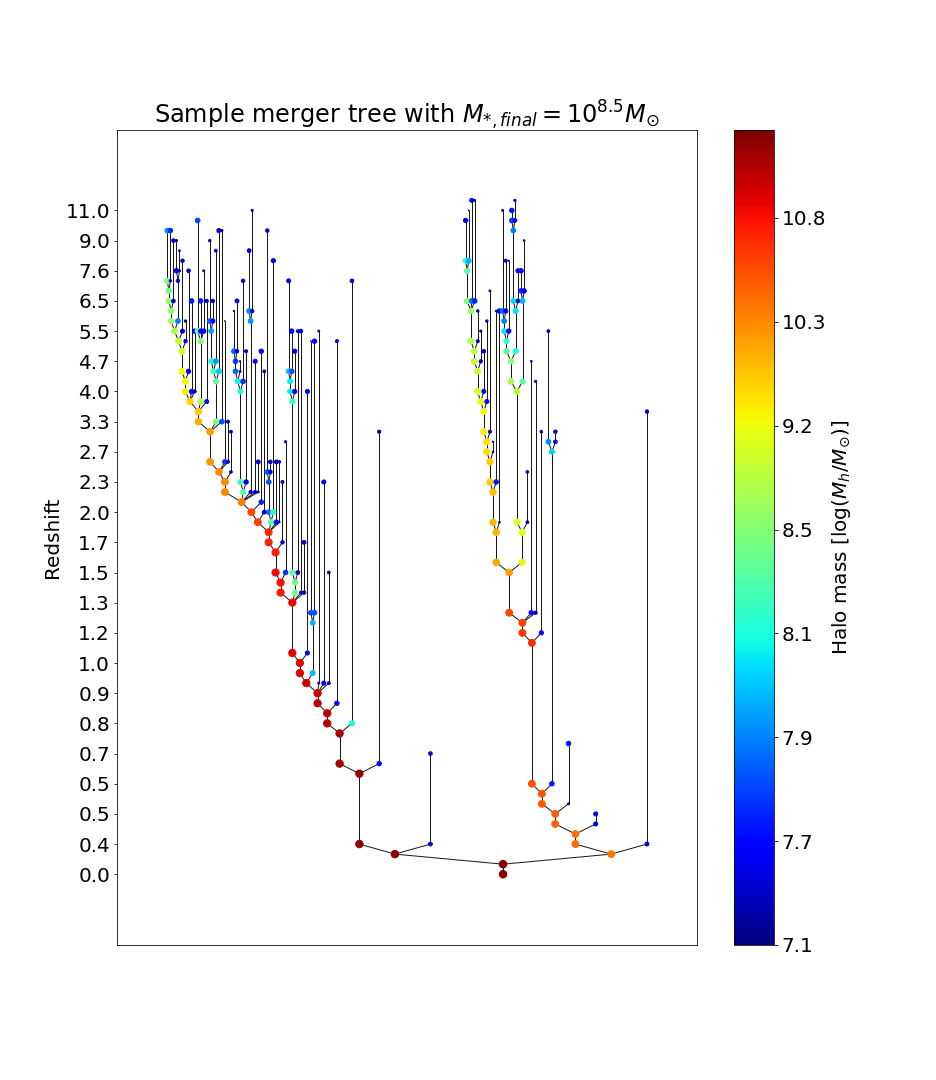
\includegraphics[width=0.7\textwidth]{figures/full_tree2}
\caption{A dark-matter halo merger tree: the assembly history is a graph by
construction, with nodes coloured by halo mass and edges following the flow of
time.}
\label{fig:merger_tree}
\end{figure}

\begin{figure}[t]
\includegraphics[width=\textwidth]{figures/cosmic_graph1}
\caption{The cosmic web as a proximity graph over halos: the connectivity
\emph{is} the geometry.}
\label{fig:cosmic_web}
\end{figure}


%%%%%%%%%%%%%%%%%%%%%%%%%%%%%%%%%%%%%%%%%%%%%%%%%%%%%%%%%


\section{Graph Neural Networks}
\label{sec:gnn}

A graph neural network rests on one idea, repeated: pass messages along the
edges, aggregate them, update the node. Everything else is variation on that
theme. We open with the anatomy of a single layer --- and its disguise as a
force law --- then catalogue the common layers, the tasks they serve, and the
modules from which any of the rest can be assembled.

\subsection{The anatomy of a message-passing layer}
\label{sec:message-passing}

A single message-passing layer does three things, and a physicist has done them
all before. Each node gathers messages from its neighbours, a
permutation-invariant aggregator sums them, and the node updates its state from
its own features and from the aggregate:
\[
  \mathbf{h}_u \;=\; \phi\!\Big(\mathbf{x}_u,\ \bigoplus_{v\in\mathcal{N}(u)}
        \psi(\mathbf{x}_u,\mathbf{x}_v,\mathbf{e}_{uv})\Big).
\]
At its simplest the layer reads $\mathbf{v}_i' = \mathbf{W}_1\mathbf{v}_i +
\mathbf{W}_2\,\mathrm{mean}_{j\in\mathcal{N}(i)}\mathbf{v}_j$
\citep{Hamilton2017_GraphSAGE_inductive,Jespersen2022_mangrove}. The form should
look familiar, because it is a gravitational $N$-body update in disguise. Step
the velocity of body $i$ forward and the contributions of all other masses
simply superpose:
\[
  \mathbf{v}_i^{t+1} \;=\; \mathbf{v}_i^{t}
    + \Delta t \sum_{j\neq i}
      \frac{G\,m_j(\mathbf{x}_j^{t}-\mathbf{x}_i^{t})}
           {|\mathbf{x}_j^{t}-\mathbf{x}_i^{t}|^{3}} .
\]
The carry-forward term plays the role of $\phi(\mathbf{x}_u,\cdot)$; the pairwise
pull $G m_j(\mathbf{x}_j-\mathbf{x}_i)/r^3$ is the edge message $\psi$; the sum
over bodies is the aggregator; the leading ``$+$'' is the residual update. A
GNN layer, then, is a learnable, generalised force law plus a one-step
integrator --- which is why message passing feels native to physicists, and why
the learned edge function so often reads back as a physical force
\citep{Cranmer2019_symbolicphysics_GNN,Lemos2023_orbitalmechanics_symbolic}.

\subsection{Common propagation layers}
\label{sec:flavours}

The propagation layer comes in three canonical flavours
\citep{Bronstein2021_geometricDL_book,Velickovic2022_messagepassing_up}, in
order of rising expressivity --- and of rising cost. With aggregator
$\bigoplus$ and learnable maps $\psi,\phi$:
\begin{align}
\text{Convolutional:}\quad
  \mathbf{h}_u &= \phi\!\Big(\mathbf{x}_u, \textstyle\bigoplus_{v\in\mathcal{N}_u}
       c_{vu}\,\psi(\mathbf{x}_v)\Big), \\
\text{Attentional:}\quad
  \mathbf{h}_u &= \phi\!\Big(\mathbf{x}_u, \textstyle\bigoplus_{v\in\mathcal{N}_u}
       a(\mathbf{x}_u,\mathbf{x}_v)\,\psi(\mathbf{x}_v)\Big), \\
\text{Message passing:}\quad
  \mathbf{h}_u &= \phi\!\Big(\mathbf{x}_u, \textstyle\bigoplus_{v\in\mathcal{N}_u}
       \psi(\mathbf{x}_u,\mathbf{x}_v,\mathbf{e}_{uv})\Big).
\end{align}
The convolutional layer fixes the neighbour weights $c_{vu}$ (GCN); the
attentional layer learns a scalar weight $a(\mathbf{x}_u,\mathbf{x}_v)$ (GAT);
message passing computes a full vector message per edge (MPNN). To descend the
list is to buy expressivity with parameters and compute
(Fig.~\ref{fig:flavours}).

\begin{figure}[t]
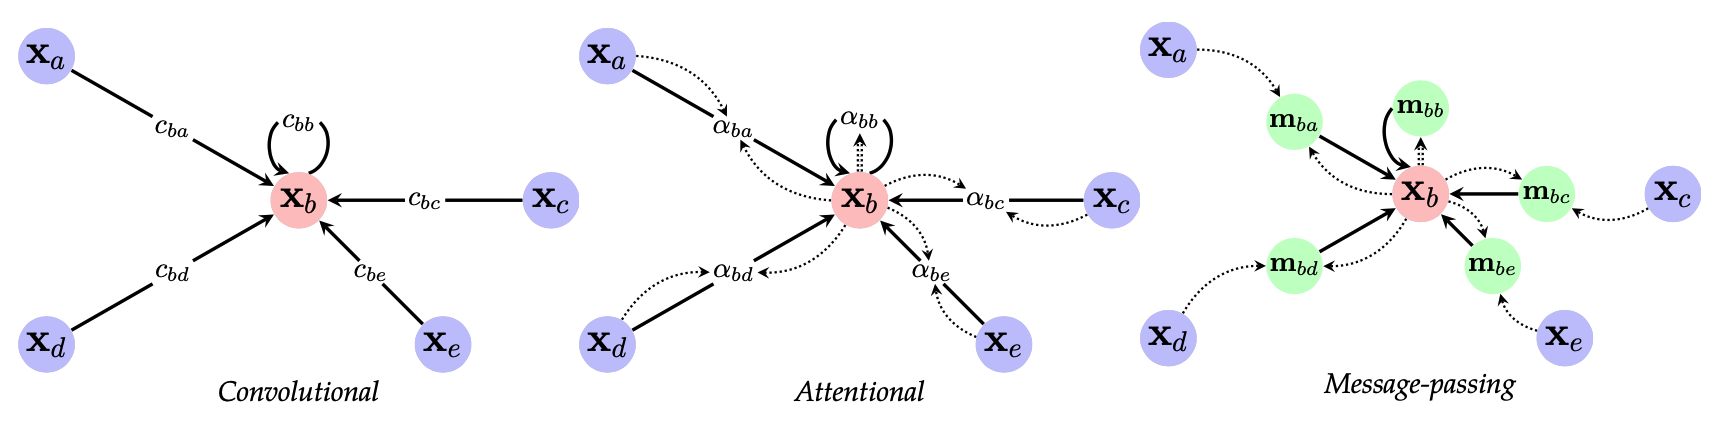
\includegraphics[width=\textwidth]{figures/bronstein_layer_overview}
\caption{TODO --- MAKE OWN VERSION (placeholder lifted from
\citealp{Bronstein2021_geometricDL_book}; replace before publication). Dataflow
for the three flavours of GNN layer, on the neighbourhood of node $b$. Left to
right: convolutional ($c_{uv}$ fixed); attentional
($\alpha_{uv}=a(\mathbf{x}_u,\mathbf{x}_v)$); message passing
($\mathbf{m}_{uv}=\psi(\mathbf{x}_u,\mathbf{x}_v)$).}
\label{fig:flavours}
\end{figure}

\subsection{Prediction types}
\label{sec:tasks}

A graph affords every task one might want, across three levels and two modes:
node, edge, and graph, in classification or regression
(Fig.~\ref{fig:tasks}). On the cosmic web alone one may ask, at the graph level,
whether a volume comes from a universe beyond $\Lambda$CDM, or what its $\Omega_m$
is; at the node level, whether the galaxy in a halo is quiescent, or what its
stellar mass is; at the edge level, whether two halos will merge, and in how
long. Node- and edge-level outputs demand permutation \emph{equivariance};
graph-level outputs demand permutation \emph{invariance}.

\begin{figure}[t]
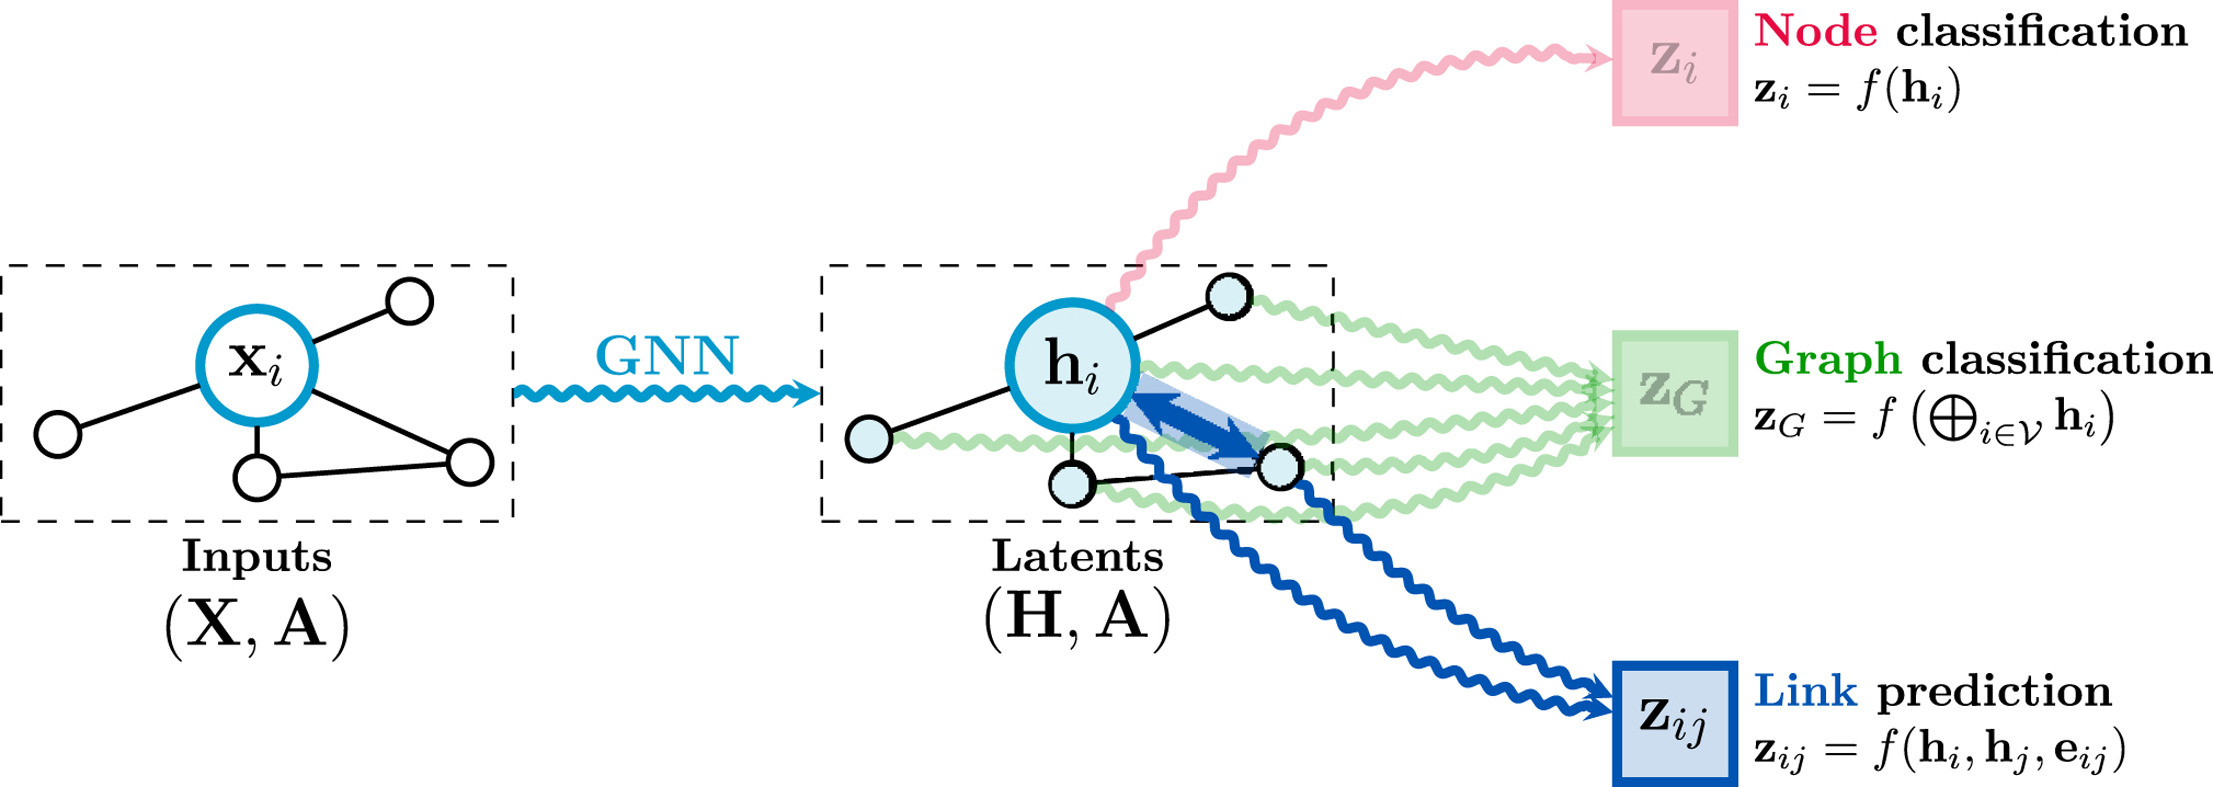
\includegraphics[width=\textwidth]{figures/velickovic_tasks}
\caption{The task taxonomy: node-, edge-, and graph-level prediction (each in
classification or regression). After \citet{Velickovic2023_everythingconnected_review}.}
\label{fig:tasks}
\end{figure}

\subsection{Composing edge, node, and global features into one layer}
\label{sec:compose}

The three feature types --- edge, node, and global --- need not act in
isolation; a full layer updates each in turn and lets information flow between
them (Fig.~\ref{fig:workflow}). One updates edges from their endpoints, then
nodes from their aggregated edges, then the global feature from the whole. This
order is a convention, not a law, but it composes the relational, the local, and
the global into a single, permutation-respecting operation.

\begin{figure}[t]
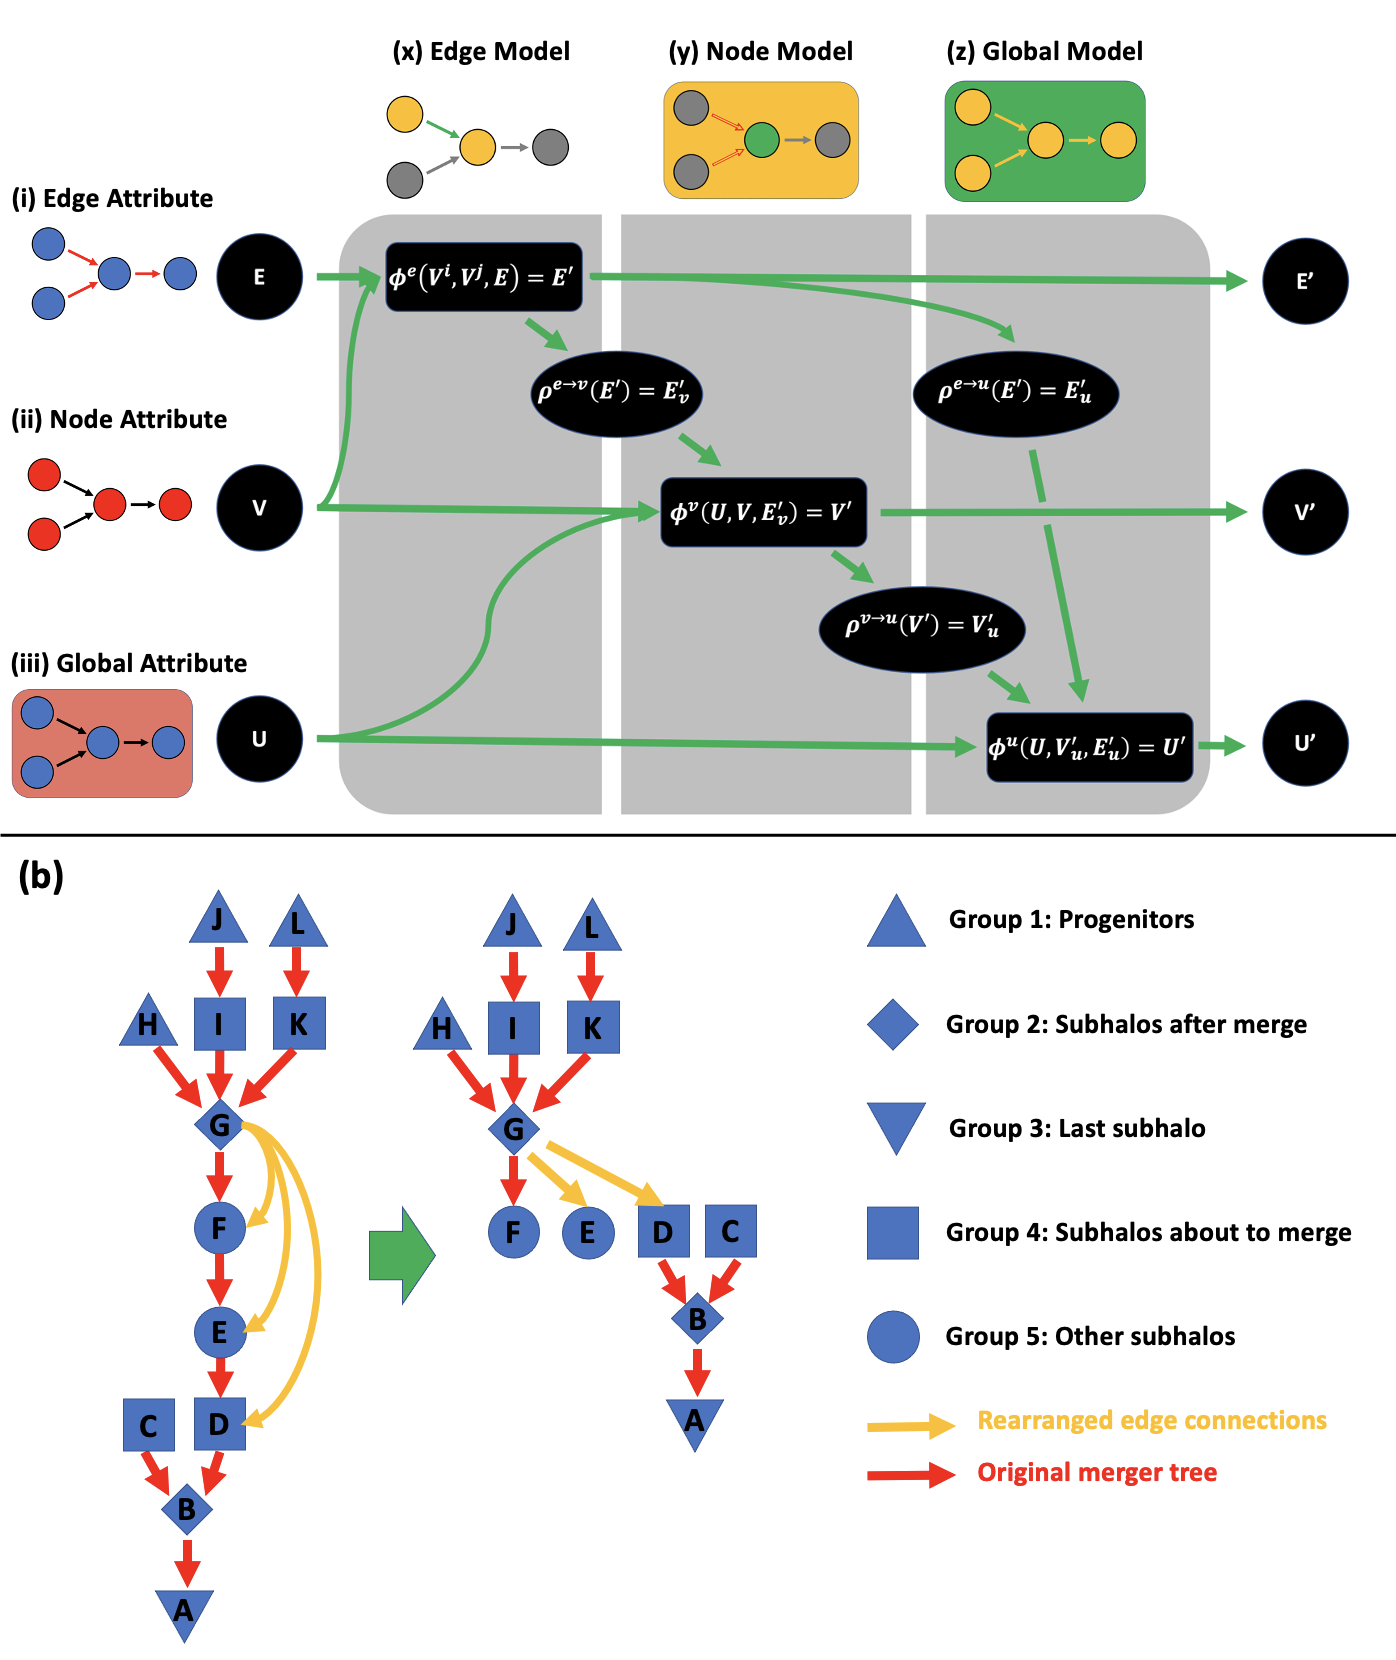
\includegraphics[width=\textwidth]{figures/workflow}
\caption{How to compose edge, node, and global features into a single graph
network layer: edges update from their endpoints, nodes from their incident
edges, and the global feature from the whole graph.}
\label{fig:workflow}
\end{figure}

\subsection{Pooling and readout}
\label{sec:pooling}

To turn node features into a graph-level answer, one pools. The simplest
readouts sum, average, or take the maximum over nodes --- order-independent, and
so permutation-invariant \citep{VillanuevaDomingo2022_cosmicgraph_clustering}.
Richer, distribution-aware readouts exist: a differentiable histogram, for one,
captures higher moments and stays interpretable in the language of classical set
summaries \citep{Cranmer2021_histpool_deepsets}. Hierarchical pooling instead
coarsens the graph in stages \citep{Ying2018_diffpool_pooling}. The aggregator
is best read as any statistically meaningful summary of the neighbourhood ---
minimum, maximum, mean, variance, and onwards.

\subsection{Scaling up: sampling}
\label{sec:sampling}

When a graph grows to millions of nodes, one cannot pass messages over all of it
at once. Sampling controls the cost --- by node, by layer, or by subgraph ---
and trades exactness for tractability, the price of working at survey scale.

\subsection{The computational-modules zoo}
\label{sec:zoo}

The literature offers dozens of propagation layers, samplers, and pooling
operators; PyTorch Geometric alone lists some sixty-five. Their number need not
intimidate. Once one grasps the few principles behind the common layers, any of
the rest is a short step away --- the knowledge of certain principles, again,
supplying the knowledge of certain facts. Figure~\ref{fig:modules} organises a
useful astrophysical subset as a taxonomy of computational modules.

\begin{figure}[t]
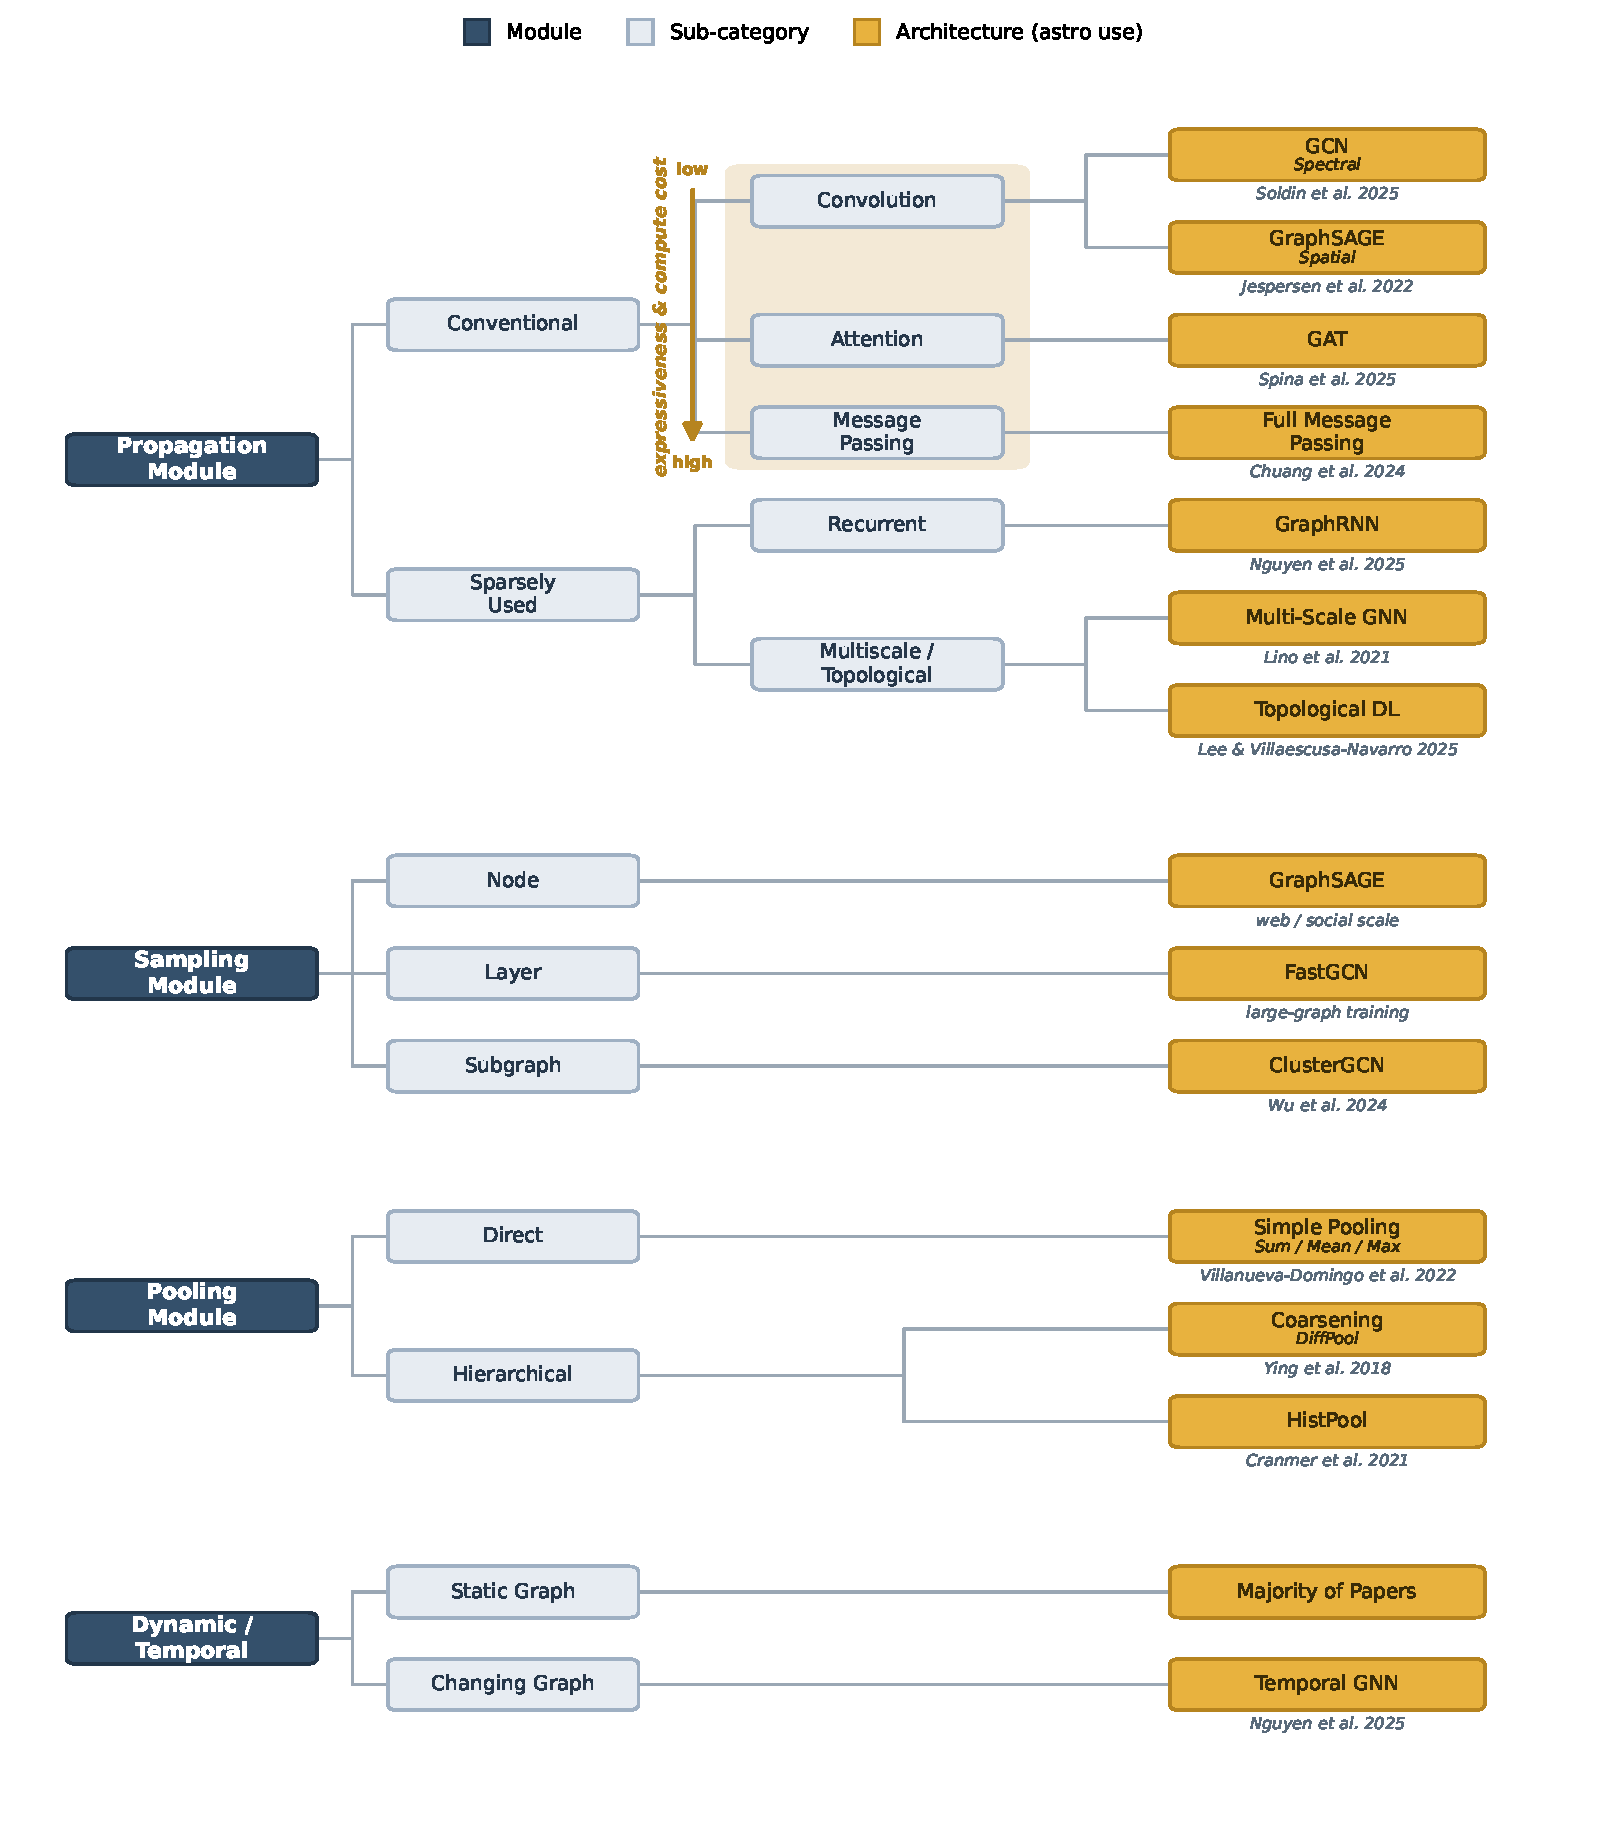
\includegraphics[width=\textwidth]{figures/computational_modules}
\caption{A taxonomy of GNN computational modules, restricted to an
astrophysically useful subset, with a representative reference on each leaf.
Adapted in the spirit of \citet{2018arXiv181208434Z}.}
\label{fig:modules}
\end{figure}


%%%%%%%%%%%%%%%%%%%%%%%%%%%%%%%%%%%%%%%%%%%%%%%%%%%%%%%%%


\section{Applications in Astrophysics and Cosmology}
\label{sec:applications}

GNNs have spread across astrophysics wherever the data refuse a grid. We
organise the survey by subfield, and we flag the honest divide between results
on real data and results that so far live only in simulation. The list is
illustrative, not exhaustive.

\subsection{Cosmology and large-scale structure}
\label{sec:app-cosmo}
Cosmology supplies the largest graphs we have. Where the likelihood is
intractable, a GNN reads parameters straight from the catalogue: cosmic graphs
over halos and galaxies constrain $\Omega_m$ and the clustering amplitude
\citep{Makinen2022_cosmicgraph_LSS, VillanuevaDomingo2022_cosmicgraph_clustering,
Shao2023_omegam_universalequation, Yang2023_haloclustering_graph}, and
field-level likelihood-free inference reads cosmology directly from galaxy
positions \citep{deSanti2023_fieldlevel_LFI}. Point clouds of dark-matter halos
yield parameters \citep{Chatterjee2025_pointcloud_cosmology}, discrete tracers
are lifted back to continuous fields \citep{Kvasiuk2024_fieldreconstruction_GNN},
and the cosmic web is classified by environment
\citep{Kololgi2025_cosmicweb_classification}. Robustness across surveys and
simulations drives domain adaptation \citep{Roncoli2023_domainadaptation_cosmology,
Lee2024_SDSS_domaingeneralization}, while topological deep learning
\citep{Lee2025_topological_cosmology}, graph-based CMB recovery
\citep{Adams2023_CMB_graphconv}, Bayesian lensing inference
\citep{Park2023_lensing_bayesianGNN}, primordial non-Gaussianity
\citep{Jung2023_QuijotePNG_massfunction}, and cosmic-void finding with graph
flows or differentiable histograms \citep{Thiele2026_void_graphflow,
Cranmer2021_histpool_deepsets} fill out the field. Common benchmarks have begun
to appear \citep{Huang2025_CosmoBench_benchmark}.

\subsection{Galaxy formation and the galaxy--halo connection}
\label{sec:app-galaxies}
The bond between a galaxy and its dark-matter halo is relational, and the merger
tree makes it a graph. \texttt{Mangrove} maps merger trees onto galaxy
properties orders of magnitude faster than a semi-analytic model
\citep{Jespersen2022_mangrove}, and later work leaves no branch behind
\citep{Chuang2024_mergertree_GNN}. The galaxy--environment connection is learned
directly \citep{Wu2023_galaxyenvironment_GNN, Wu2024_galaxyhalo_environment,
Jespersen2026_environment_assembly}, halo masses are inferred from their
neighbourhoods \citep{VillanuevaDomingo2022_halomass_GNN,
Larson2024_halomass_images}, and intrinsic alignments --- a vector quantity ---
are modelled equivariantly \citep{Jagvaral2022_intrinsicalignment_GNN}. Clusters
are weighed from 2D observables and X-ray profiles
\citep{Delgado2025_cluster_triaxiality, Iqbal2025_cluster_xray_GNN}, and
generative models now emulate assembly histories and subhalo populations
\citep{Roper2020_MEGA_mergergraph, Nguyen2024_FLORAH_assembly,
Nguyen2025_mergertree_generative, Nguyen2026_DREAMS_diffusion}.

\subsection{Dynamics}
\label{sec:app-dynamics}
Dynamics is where the force-law analogy of Sect.~\ref{sec:message-passing}
becomes literal. Interaction networks learn the equations of motion of $N$-body
systems and, through symbolic regression, hand them back as readable laws
\citep{Cranmer2019_symbolicphysics_GNN, Cranmer2020_symbolicregression_inductivebias,
Lemos2023_orbitalmechanics_symbolic}. The same machinery predicts the stability
of compact planetary systems \citep{Cranmer2021_planetarystability_BNN} and
reconstructs galaxy mergers with equivariant flows
\citep{Tang2022_merger_normalizingflow}; the broader programme of learned
simulators \citep{SanchezGonzalez2020_GNS_physics, Pfaff2020_meshsim_GNN} waits
to be turned loose on astrophysics in earnest.

\subsection{Detectors and instrumentation}
\label{sec:app-instruments}
Detectors rarely sit on grids, and neutrino telescopes least of all. GNNs
reconstruct IceCube events faster and more precisely than the classical pipeline
\citep{Choma2018_IceCube_classification, Abbasi2022_IceCube_lowenergy,
Soldin2025_IceCube_GCN, Jespersen2022_icecube_bachelor}, an effort now
consolidated in the \texttt{GraphNeT} library and its benchmarks
\citep{Sogaard2023_graphnet_neutrino, Orsoe2025_graphnet2_library,
Orsoe2026_nubench_benchmark, Bukhari2023_icecube_kaggle} and carried to
IceCube-Gen2 and IceAct \citep{VaraCarbonell2025_IceCubeGen2_ML,
Paul2025_IceAct_spectrum}. Cosmic-ray observatories follow
\citep{Rodriguez2025_Auger_photon, Ferriere2025_GRAND_cosmicray}, interferometers
are simulated on graphs \citep{Kannan2025_interferometer_GNN}, and the scheduling
of the telescopes themselves --- a combinatorial graph problem --- yields to the
same tools \citep{Wang2022_spectroscopy_resourceallocation,
Cranmer2021_resourceallocation_unsupervised}.

\subsection{Stellar populations, the Milky Way, and dark-matter substructure}
\label{sec:app-stellar}
Closer to home, GNNs sort stars and probe the dark sector. Chemical tagging ---
the attempt to reunite stars born together --- is recast as a graph problem,
through attention over abundances \citep{Spina2025_chemicaltagging_GAT} and
through graph kernels \citep{Ting2023_WLkernel_chemicaltagging}. Substructure in
the Milky Way halo emerges from Gaia and APOGEE
\citep{Berni2025_MWhalo_substructure}, the masses of the Milky Way and Andromeda
are inferred from their satellites \citep{VillanuevaDomingo2023_MW_mass}, and the
density profiles of dwarf galaxies --- a direct handle on dark matter --- are
uncovered with graph networks \citep{Nguyen2023_dwarf_densityprofile,
Nguyen2025_dwarf_GraphNPE}.


%%%%%%%%%%%%%%%%%%%%%%%%%%%%%%%%%%%%%%%%%%%%%%%%%%%%%%%%%


\section{Best Practices}
\label{sec:bestpractices}

Principles guide; practice decides. This section gathers the hard-won, sometimes
deflating advice that the rest of the chapter implies: which layers to try
first, when to leave the graph on the shelf, how to bake in what we already
know, and how to read the literature without being fooled.

\subsection{Choosing an architecture}
\label{sec:bp-choose}
For a first attempt, message passing and \texttt{SAGEConv} layers are almost
always a sound start; attention layers tend to train unstably, and plain graph
convolution is often too inexpressive. For the aggregator, begin with a sum or a
maximum, or simply concatenate several. These are starting points, not
commandments.

\subsection{When not to use a graph}
\label{sec:bp-when-not}
A graph is the wrong tool for data that already carry more structure. Regular,
evenly sampled one-dimensional sequences, images on a grid, and very large
datasets of very large graphs each have more efficient homes --- though we note
that it is \emph{regularity}, not low dimension, that decides: irregular
sequences of varying length sit naturally on a graph
\citep{Iqbal2025_cluster_xray_GNN}. Two further cautions. Very deep GNNs risk
\emph{oversmoothing}, in which repeated message passing washes node
representations toward a common value; residual connections, normalisation, or
simple restraint help. And GNNs are not cheap: the price of their generality,
of the few assumptions they make about domain or signal, is a heavier compute
bill than a structure-exploiting model would pay.

\subsection{Embedding inductive biases}
\label{sec:bp-bias}
Do not learn what you already know. We learn faster, cheaper, and more robustly
when we hand the model the structure we trust --- through the symmetries we
build in, and through the graph we construct (time resolution, locality,
causality)\citep{Jespersen2022_mangrove,Chuang2024_mergertree_GNN,
Jespersen2026_environment_assembly}. None of this forbids a flexible model from
finding the same solution; it merely spares it the trouble. A graph is itself
so strong a prior that a wrong one misleads
\citep{BechlerSpeicher2023_graph_overuse}, and where a symmetry holds only
approximately, a soft constraint can outperform a hard one, at the cost of
softer guarantees \citep{Finzi2021_RPP_softequivariance}.

\subsection{Pitfalls, diagnostics, and validation}
\label{sec:bp-diagnostics}
% TODO: expand. False invariance/equivariance claims; sim->real shift;
% sensitivity to the chosen adjacency; verification in the spirit of SBI
% diagnostics \citep{Thiele2026_SBI_review}.

\subsection{Reading the astro-GNN literature}
\label{sec:bp-reading}
A short field guide. Look for two things: a direct line from the problem to the
architecture, geometry, and inductive biases it invokes; and a real gain, in
performance or interpretability, over simpler baselines. Be wary of two red
flags: claimed invariances or equivariances the model does not possess, and
graphs deployed where a grid or a sequence would serve better. In short, the
graph should earn its place.


%%%%%%%%%%%%%%%%%%%%%%%%%%%%%%%%%%%%%%%%%%%%%%%%%%%%%%%%%


\section{Frontier}
\label{sec:frontier}

The frontier runs wherever astrophysics outgrows point-wise statistics, and we
flag a few directions. \emph{Generative} graph models remain hard, and largely
unproven on astrophysical data, yet merger-tree and field generation already
press on the question \citep{Nguyen2024_FLORAH_assembly,
Nguyen2025_mergertree_generative,Tang2022_merger_normalizingflow,
Onutu2025_scorematching_cosmology}. \emph{Geometric graphs}, whose nodes carry
coordinates and whose symmetry is therefore spatial as well as permutational,
promise a more interpretable handle on large-scale structure, at the price of
the extra equivariances one must respect \citep{Lee2025_topological_cosmology,
GarciaSatorras2021_EGNN_equivariant}. \emph{Temporal} GNNs, on changing graphs,
fit the time-ordered data of assembly and of transient surveys. And simulation-
based inference, the subject of a companion chapter, marries naturally to GNNs
that learn summaries of genuinely graph-structured data
\citep{Thiele2026_SBI_review} --- a direction we look forward to pursuing on
real data ourselves.


%%%%%%%%%%%%%%%%%%%%%%%%%%%%%%%%%%%%%%%%%%%%%%%%%%%%%%%%%


\section{Tutorials}
\label{sec:tutorials}

Theory carries only so far; the reader who wishes to experiment will find a
hands-on GNN tutorial at \url{https://tinyurl.com/GNN1tutorial} and a companion
competition --- on the connection between a galaxy and its environment --- at
\url{https://tinyurl.com/GNNcompetition}. Beyond these, three external resources
repay the visit: the interactive ``Gentle Introduction to Graph Neural
Networks'' on Distill; the Stanford CS224W course with its Colab notebooks; and
the geometric-deep-learning proto-book and lectures of
\citet{Bronstein2021_geometricDL_book}.


%%%%%%%%%%%%%%%%%%%%%%%%%%%%%%%%%%%%%%%%%%%%%%%%%%%%%%%%%


\section{Summary and Outlook}
\label{sec:summary}
% DRAFT -- CKJ to review before we finalise.

We set out to teach a principle, not a catalogue. Physics advances by geometry,
and the algorithms we build for it ought to do the same: fit the structure the
data actually have, respect the symmetries we already trust, and learn only what
remains. The geometric blueprint turns this conviction into a recipe, and the
graph neural network is its most general instrument --- the one from which
convolutional networks, transformers, and deep sets all fall out as special
cases.

Three threads run through the chapter. First, geometry: weigh the native
structure of both the domain and the signal before you reach for an
architecture. Second, the graph: a relational substrate that fits merger trees,
detectors, and the cosmic web where a grid never will, and whose adjacency is a
design choice we set from physics or learn. Third, the graph neural network:
message passing as a learnable force law, assembled from a handful of layers and
aggregators that the reader can now read off and adapt at will.

The strength of the approach lies not in symmetry, prior knowledge, or
flexibility alone, but in the three held together. A graph neural network lets
us bake in the symmetries and the structure we trust while we stay free to fit
what we do not yet understand --- and it speaks, throughout, the native language
of physics: objects, and the relations between them.

The frontier is wide and largely open: generative models of cosmic structure,
geometric graphs for the web, temporal graphs for an evolving and transient sky,
and simulation-based inference on real, graph-structured data. The tools are
ready; the Universe, as ever, is under no obligation to be simple.


%%%%%%%%%%%%%%%%%%%%%%%%%%%%%%%%%%%%%%%%%%%%%%%%%%%%%%%%%


% ===================== APPENDICES =====================
% Springer: end-of-chapter appendices use the heading "Appendix" (no \appendix).
% =====================================================================
% DRAFT APPENDIX: Symmetries, Representations, and Invariance
% Rewritten (NOT lifted) from Bronstein et al. (2021) GDL proto-book, sec. 3
% \citep{Bronstein2021_geometricDL_book}, per CKJ margin comment p.16.
% Depth: EXPANSIVE on 3.1, SHORT on 3.2 & 3.3, MEDIUM on 3.4; 3.5 (the
% blueprint) lives in the main text. House style: light on abstract math,
% heavy on physical-system analogies. Group-theory statements refer to
% \citep{Bronstein2021_geometricDL_book} and/or Zee's "Group Theory in a
% Nutshell for Physicists" \citep{Zee2016_grouptheory_nutshell}; other
% citations (Klein's Erlangen Programme, Mallat for wavelets) replicated from
% Bronstein and can be promoted to bib entries if we keep them.
% TODO (CKJ): revisit this appendix later -- run-in headings (svmult \runinhead
% vs orphaned \paragraph), the subsection title duplicating the section title,
% and general structure/typography.
% =====================================================================

\section{Appendix: Symmetries, Representations, and Invariance}
\label{app:symmetries}

This appendix collects the geometric vocabulary the main text leans on. We follow the framing of \citet{Bronstein2021_geometricDL_book}, but keep the mathematics light and the physics close; readers wanting the full group-theory machinery will find a physicist-friendly treatment in \citet{Zee2016_grouptheory_nutshell}.

\subsection{Symmetries, representations, and invariance}
\label{app:sym:basics}

A \emph{symmetry} is a transformation that leaves some property of a system unchanged. Physicists meet symmetries before they meet the word: the outcome of an experiment does not depend on \emph{where} the bench sits (translation), \emph{which way} it faces (rotation), or \emph{when} it is run (time translation); a molecule's energy does not care how the molecule is oriented; a set of identical particles does not care in what order we list them. Each ``does not care'' is a symmetry, and -- as Noether taught us -- each continuous one is shadowed by a conserved quantity.

Symmetries compose: doing one and then another is again a symmetry, every symmetry can be undone, and ``do nothing'' is a symmetry. Those three facts are exactly the axioms of a \emph{group}, the natural home for a system's symmetries. We keep the definition formal, since everything else hangs off it:

\begin{definition}[Group]
A \emph{group} is a set $G$ with a composition rule
$\circ : G\times G \to G$ (written $g\circ h = gh$) obeying:
\begin{itemize}
  \item \textbf{Associativity:} $(gh)k = g(hk)$ for all $g,h,k\in G$;
  \item \textbf{Identity:} a unique $e\in G$ with $eg = ge = g$ for all $g$;
  \item \textbf{Inverse:} each $g$ has a unique $g^{-1}$ with $gg^{-1}=g^{-1}g=e$;
  \item \textbf{Closure:} $gh\in G$ for all $g,h\in G$.
\end{itemize}
\end{definition}

Commutativity is \emph{not} required: in general $gh \neq hg$ (rotating then translating differs from translating then rotating). Groups for which $gh=hg$ always hold are called \emph{Abelian}. Large groups are often built from a handful of \emph{generators} -- e.g.\ the symmetries of an equilateral triangle are generated by one rotation and one reflection, and that same six-element group is also the group of permutations of three labelled corners. This little coincidence is the seed of a recurring theme: the \emph{same} abstract group can act on very different objects.

\paragraph{Group actions and representations.} We rarely care about a group in the abstract; we care about how it \emph{acts} on our data. If the group acts on the underlying domain $\Omega$ (rotating points in space, relabelling nodes of a graph), it automatically acts on signals defined over that domain (rotating an image, permuting node features). The actions that matter for us are \emph{linear}, and a linear action is precisely a \emph{representation}: a rule $\rho$ that assigns to each group element $g$ an invertible matrix $\rho(g)$ such that $\rho(gh)=\rho(g)\rho(h)$ -- composing transformations becomes multiplying matrices. The physicist's reflex is the right one here: this is exactly how a scalar, a vector, or a higher tensor ``transforms under rotation'' (the rotation matrices, or for higher spins the Wigner $D$-matrices), and the dimension of $\rho$ is just the size of the feature it acts on, not of the group itself. (\citealp{Zee2016_grouptheory_nutshell} develops representations from this physical standpoint.)

\paragraph{Invariance vs.\ equivariance.} Imposing a symmetry on a learned function $f$ is a powerful inductive bias: it shrinks the space of candidate functions to those that already respect the symmetry, so less has to be learned from data. Two cases recur throughout the review:

\begin{definition}[Invariance and equivariance]
A function $f$ is \emph{$G$-invariant} if $f(\rho(g)x) = f(x)$ for all $g\in G$ -- the output ignores the transformation. It is \emph{$G$-equivariant} if $f(\rho(g)x) = \rho(g)\,f(x)$ -- the output transforms in lockstep with the
input.
\end{definition}

The physical reading is immediate. A molecule's total energy is rotation- and permutation-\emph{invariant} (rotate the molecule, relabel its atoms -- the energy is unmoved); the force on each atom is rotation-\emph{equivariant} (rotate the molecule and every force vector rotates with it) and permutation-\emph{equivariant} (relabel the atoms and the list of forces is relabelled the same way). The same split organizes graph tasks: a graph-level prediction should be permutation-invariant, while node- and edge-level predictions should be permutation-equivariant. Convolutional layers are the canonical equivariant building block -- shifting the input shifts the output feature map by the same amount -- and a final global pooling turns equivariance into invariance. That ``stack equivariant layers, then pool'' pattern is the geometric-deep-learning blueprint discussed in the main text.

\subsection{Levels of structure: isomorphisms and automorphisms}
\label{app:sym:iso}

What counts as a symmetry depends on \emph{how much structure} we insist on preserving. A bare set only has a size, so its symmetries are all relabellings (bijections). Demand that nearness be preserved and you keep only continuous maps; demand smoothness, only diffeomorphisms; demand distances, only \emph{isometries} (rotations, translations, reflections). Each extra requirement carves out a \emph{subgroup} of the previous group: more structure preserved means fewer allowed transformations. This nesting is exactly Klein's Erlangen-Programme view of geometry (projective $\supset$ affine $\supset$ Euclidean), and it is the lens we use to decide which symmetries a given astrophysical problem actually has.

One distinction is worth stating plainly because it is routinely blurred. An \emph{automorphism} maps an object to \emph{itself} while preserving its structure -- this is what we have been calling a symmetry. An \emph{isomorphism} maps between \emph{two different} objects that are structurally the same. For graphs this is the everyday statement that two graphs are ``the same graph drawn differently'': a graph isomorphism is a node relabelling that preserves every connection (and non-connection), while a graph \emph{automorphism} is such a relabelling of a graph onto itself -- a genuine internal symmetry. This is the precise sense in which a GNN's permutation symmetry says ``the labels are arbitrary; only the relations matter.''

\subsection{Deformation stability: when symmetries are only approximate}
\label{app:sym:deformation}

Exact symmetries are an idealization. The real world is noisier: in a video, several objects each drift their own way, so no single global shift relates consecutive frames; a galaxy image may be mildly warped by lensing or seeing yet still show the same galaxy. What we really want is not exact invariance to a clean group, but \emph{approximate} invariance to transformations that are \emph{close} to that group. The fix is to measure how far a transformation $\tau$ sits from the symmetry group $G$ with a cost $c(\tau)$ (zero on $G$ itself) and to ask only for \emph{deformation stability},
%
\begin{equation}
\| f(\rho(\tau)x) - f(x)\| \;\le\; C\,c(\tau)\,\|x\|,
\label{eq:def-stability}
\end{equation}
%
i.e.\ small deformations may change the output, but only a little. (Small deformations cannot simply be added to the group, because composing many small ones makes a large one -- they do not close.) This is the formal version of a demand we make repeatedly: a good model should degrade gracefully, not catastrophically, when the symmetry it assumes holds only approximately, and it connects to the \emph{soft}-constraint idea (imposing a symmetry as a prior rather than a hard architectural law).

The same idea applies when it is the \emph{domain}, not the signal, that deforms -- the case closest to our subject. A social or follow graph changes its edges over time; the cosmic web is a different graph at every redshift; a 3D shape flexes. One quantifies these by a distance between domains (e.g.\ graph edit distance, which vanishes for isomorphic graphs, or the Gromov--Hausdorff distance for manifolds) and asks that $f$ change slowly in that distance.

\subsection{Scale separation}
\label{app:sym:scale}

Deformation stability tames \emph{local} wobble, but on a large domain there are still far too many stable functions to learn efficiently -- the curse of dimensionality bites. The escape is \emph{scale separation}: most physical tasks are organized hierarchically, so we can build global understanding by composing local, multi-scale pieces.

The classical tool for ``which scales are present'' is the Fourier transform, which rewrites a signal as a sum of oscillations indexed by frequency, and which turns convolution into simple multiplication (the convolution theorem). Fourier descriptors capture \emph{global} properties (smoothness, overall power) and are perfectly matched to a clean global symmetry like translation -- the modulus of the Fourier transform, for instance, is exactly shift-invariant. But Fourier representations are \emph{fragile}: an arbitrarily small, high-frequency deformation can change them by an order-one amount, because each basis function is spread over the whole domain.

\emph{Wavelets} (and multi-scale representations generally) repair this by using filters localized in \emph{both} space and scale: fine details are captured by small-support atoms, coarse trends by large-support ones. Crucially, a multi-scale decomposition is approximately \emph{equivariant} to deformations (its error grows like the deformation size, $O(\epsilon)$, rather than $O(1)$), turning a globally unstable description into a family of locally stable features. Those features are not yet invariant; they must be combined progressively from fine to coarse -- which is precisely why useful architectures are \emph{deep} and \emph{hierarchical}, interleaving local operators with coarsening. The astrophysical resonance is hard to miss: structure formation, turbulence, and the cosmic web are all multi-scale, and a model that respects scale separation is matching the physics of its inputs. (See \citealp{Bronstein2021_geometricDL_book} and references therein, e.g.\ Mallat on wavelets, for the technical development.)

The graph inherits every piece of this story through the \emph{graph Laplacian} $L = D - A$, with $D$ the diagonal matrix of node degrees. $L$ acts as the discrete second derivative on the graph: apply it to a signal, and it returns zero wherever the signal runs smooth across the edges and large values wherever the signal jumps. Its eigenvectors are the graph's Fourier modes and its eigenvalues their frequencies, which cashes out the promise of Figure~\ref{fig:graph_anatomy} that the spectrum of $A$, or of its Laplacian, reveals communities, diffusion, and scale. Spectral graph convolutions filter in exactly this eigenbasis \citep{Bruna2013_spectral_networks, Defferrard2016_chebnet}, and the GCN of \citet{Kipf2016_GCN_semisupervised} descends from them as a fast local approximation. Message passing reaches the same operations without ever computing an eigendecomposition, which is why the main text keeps the spatial view.

% NOTE: 3.5 (the GDL blueprint: equivariant layers -> local pooling -> global
% pooling -> readout) is covered in the MAIN TEXT, not here (per CKJ).


\section{Appendix: Why a convolution is the only translation-equivariant layer}
\label{app:conv-proof}
% TODO: write the instructive derivation that a linear map commutes with all
% shifts iff it is a convolution (with the converse). Companion example: the
% Deep Sets characterisation -- permutation-invariant set functions take the
% form rho(sum phi(x_i)), and a permutation-equivariant linear layer is
% a I + b (1 1^T)/n \citep{Zaheer2017_deepsets}.


%%%%%%%%%%%%%%%%%%%%%%%%%%%%%%%%%%%%%%%%%%%%%%%%%%%%%%%%%


\bibliographystyle{spbasic}   % Springer basic author-year style
\bibliography{ref}


\end{document}
